\section{CONTAINDER Design}\label{sec:design}
% provenance: dec_01KXT28WTZ92PJ7S8D3MME78D4 (novelty framing); dec_01KXT25BXRB50HY38SZ8P9ADFD (RQ4).
% provenance: jrn_01KXTVC4CT850YTVE5EM3RJDGS (revision directive: fresh-key binding, session + command enforcement, safe mode).
% provenance: jrn_01KXT3JPAZ8RSGZK99X4G3HWPE constrains renewal to avoid online-responder/secure-time dependencies.

CONTAINDER separates the layers that IEEE~2030.5 conflates and enforces credential lifetime at
the session and command layers, not only at issuance. The design is a containment chain:
fresh attestation, a fresh hardware-bound key, a short scoped operational credential, a bounded
session, and a bounded command effect, so that removing authority actually removes control. Each
link targets a dimension of the model (Fig.~\ref{fig:chain}).

\begin{figure*}[t]
\centering
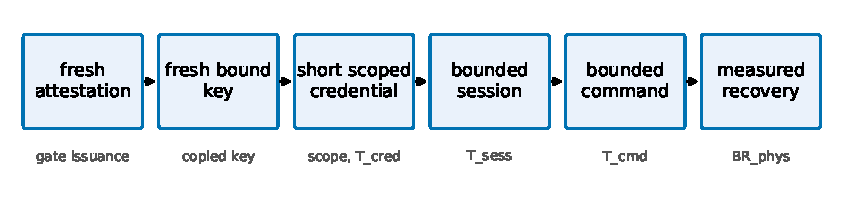
\includegraphics[width=\textwidth]{figures/fig_chain.pdf}
\caption{The CONTAINDER containment chain. Each link bounds a dimension: attestation gates
issuance, fresh-key binding contains a copied key, scope and short lifetime bound $\BRflex$ and
$T_{\mathrm{cred}}$, session and command enforcement bound $T_{\mathrm{sess}}$ and
$T_{\mathrm{cmd}}$, and measured recovery bounds $\BRphys$.}
\label{fig:chain}
\end{figure*}

\subsection{Components and trust layering}
The device keeps a long-lived, hardware-rooted bootstrap identity~\cite{ieee8021ar2018} used only for
enrollment and attestation, never accepted directly for DER control. An \emph{attester} produces
fresh evidence bound to a freshly generated operational public key; a \emph{verifier} checks
evidence against endorsement and reference values and returns an explicit result; a
\emph{credential issuer} signs a short-lived operational certificate embedding role, site, scope,
and expiry only for a valid attestation result; an \emph{authorization service} maps the
operational identity to least-privilege function-set assignments; the \emph{2030.5 server or
proxy} authenticates the operational certificate, enforces a maximum session age, and rechecks
authorization per command or at a bounded interval; a \emph{session controller} and a
\emph{command-lifecycle controller} bound authority beyond expiry; and a \emph{risk controller}
selects deny, scope narrowing, or bounded emergency renewal. We use the Entity Attestation
Token~\cite{rfc9711} under the RATS Attester/Verifier/Relying-Party model~\cite{rfc9334}, and
define a concrete EAT profile rather than treating EAT as a complete attestation protocol.

\subsection{Fresh-key binding}
Attesting a device is not sufficient: a healthy device can pass attestation while an attacker
retains a previously copied operational key. CONTAINDER therefore requires that every credential
epoch use a newly generated operational key, generated in a TPM, TEE, or secure element where
available and marked non-exportable, whose public-key digest is carried in the attestation
evidence. The issuer signs only the attested public key, refuses renewal that presents only a
prior certificate, rejects replayed evidence and reused nonces, and rotates the key even when the
device stays healthy. This is what contains a copied key across the next epoch.

\subsection{Session and command-effect enforcement}
Certificate expiry does not end an open TLS session or an already-issued long-duration control.
CONTAINDER closes sessions at credential expiry (or bounds session age to the credential TTL) and
revalidates authorization per command, and it bounds adversary-issued controls through a maximum
command duration, cancellation on containment, and safe-default restoration, with explicit
handling of scheduled DERControls. The two quantities the prototype measures are
\begin{align}
\Delta_{\mathrm{expiry}} &= t_{\text{last adv.\ command}} - t_{\text{expiry}},\\
\Delta_{\mathrm{effect}}  &= t_{\text{effect ends}} - t_{\text{expiry}},
\end{align}
each targeted to zero or a small declared bound. These are exactly the $T_{\mathrm{sess}}$ and
$T_{\mathrm{cmd}}$ components of $\BRauth$.

\subsection{Safe-mode policy}
Failure behavior is explicit rather than fail-open. The risk controller chooses among the states
in Table~\ref{tab:safemode}; no failure mode grants indefinite authority, and the safety of each
degraded state is validated under feeder conditions rather than assumed.

\begin{table}[t]
\centering
\caption{Safe-mode authorization states.}
\label{tab:safemode}
\small
\begin{tabular}{@{}p{0.24\columnwidth}p{0.34\columnwidth}p{0.30\columnwidth}@{}}
\toprule
State & Allowed & Denied \\
\midrule
Healthy & normal scoped control & out-of-scope control \\
Verification delayed & read telemetry, hold last safe schedule & new high-impact dispatch \\
Attestation uncertain & read-only, bounded emergency control & arbitrary set-points \\
Known compromise & read-only or total denial & all control \\
Issuer outage & prior low-risk scope, bounded grace & scope expansion, high impact \\
\bottomrule
\end{tabular}
\end{table}

\subsection{Migration compatibility}
We separate three compatibility levels --- \emph{protocol} (2030.5 messages stay conformant),
\emph{implementation} (unmodified client or server software can participate), and \emph{deployment}
(legacy and upgraded devices coexist) --- and claim none of them without a passing interoperability
test rather than asserting ``backward compatible.'' None has yet been tested;
Section~\ref{sec:prelim} reports interoperability as untested. Three tiers realize this: a
bootstrap-only legacy tier, a gateway-attested proxy tier where an edge gateway holds the
operational credential for downstream legacy devices, and a native device-attested tier.

\subsection{What non-renewal inherits from the constraints it cites}
% Reviewer M11: the mechanism inherits at least two of the three deficiencies it cites against OCSP.

Section~\ref{sec:threat} adopts the Sandia analysis's reasons why online revocation fails for DER:
no guaranteed connectivity, no trustworthy time on inverters, and no responsible reporting party.
Our mechanism inherits two of the three, and we state that rather than let a reader find it.

\emph{Secure time.} Expiry is a judgment about time, so an endpoint that cannot trust its clock
cannot enforce a short lifetime --- the deficiency cited against OCSP --- and a skewed device
clock would extend a ``short-lived'' credential indefinitely. So \textbf{expiry is never enforced
by the endpoint alone}: the issuer refuses renewal server-side where a trustworthy clock exists,
each renewal binds a fresh key to a verifier-supplied nonce so a replayed attestation cannot
extend authority however the clock reads, and session and command limits are monotonic counters
rather than wall-clock deadlines. A skewed clock then costs availability, not containment. We
have not measured skew.

\emph{Connectivity.} A twelve-hour lifetime means a DER losing backhaul for twelve hours loses
control authority, and rural outages of that length are routine. An aggregator that drops a fifth
of fleet controllability during a verifier outage has created a reliability hazard while closing a
security one. Safe-mode degradation to an autonomous volt-var profile exists for this reason;
whether the trade is acceptable is an operator's call. Our availability figures come from
in-process injection, not networked outages, and renewal storms are untested.

\emph{Who reports compromise.} Attestation detects only what it measures. Firmware integrity is
measurable; \textbf{a stolen operational key on a device with intact firmware passes
attestation}. Per-epoch fresh-key binding answers this, but containment latency is then not the
lifetime: with per-cycle detection probability $p$ and lifetime $T$, expected retention is $T/p$
--- twelve hours at $T{=}6$\,h, $p{=}0.5$, and equal to $T$ only at $p{=}1$. \textbf{We report
$T/p$ as the containment-latency figure of merit.} The alternative, a narrow access list on a
long-lived credential, contains a copied key only when someone notices and edits the list, which
has no bounded latency at all. Bounded beats unbounded; it does not beat instant.

\emph{Which tier is deployable.} Presenting three tiers evenhandedly would mislead: only one is
deployable within the next standards cycle. The native tier needs attestation and a trusted clock
on constrained inverter hardware; the legacy tier changes nothing. \textbf{The gateway-attested
proxy tier resolves all three inheritances at once} --- the gateway holds the credential and the
clock, attestation runs on capable hardware, downstream devices stay unmodified, and short
outages are buffered --- and it alone requires no change to already-certified endpoints. We regard
it as the deployment path.

\subsection{Implementation status}
% provenance: mis_01KXT2D8VVC1CDNT9WJ4CFGH9P (M3 spec).
The design is realized as an issuance and renewal service using real X.509 certificates and mutual
TLS, with a Python IEEE~2030.5-style client in place of the EPRI C client and structured event
logging for every credential, session, and command transition. Its security invariants and
workstation overhead are reported in Section~\ref{sec:prelim}; a native EPRI-client integration and
constrained-hardware measurements remain future work.
